% !TeX spellcheck = en_US
 
\chapter{Tools} 
In this chapter we talk about all tools we decided to test in our study because they fitted best the requirements of \cref{minimumrequire}. The first part of this chapter handles the tools we managed to install. We used a template to ease the comparison of our experience with the specific tools. The second part contains a list with tools that are not capable of running in Kubernetes. A quick explanation of what went wrong in the installation process is given.


\section{Searchlight (Icinga)}
\label{searchlight}
As in the section Icinga \ref{Icinga} described, we were not able to find a pure installation of Icinga for a cluster so we tried to install Searchlight as a backup plan.
Searchlight is a tool from the AppsCode Inc. \cite{appscode}, which is a company located in San Leandro  in California. 
Searchlight is as many other monitoring tools written in the programming language of Go.
\\
When first tried to install Searchlight over the yaml File we received errors from the Kubernetes cluster. There it says the tools is not able to bind the Port 8443. We could not figure out which application is using the port but as we tried to install the application on a fresh cluster it turns out to working fine.
\subsection{Appearance}
%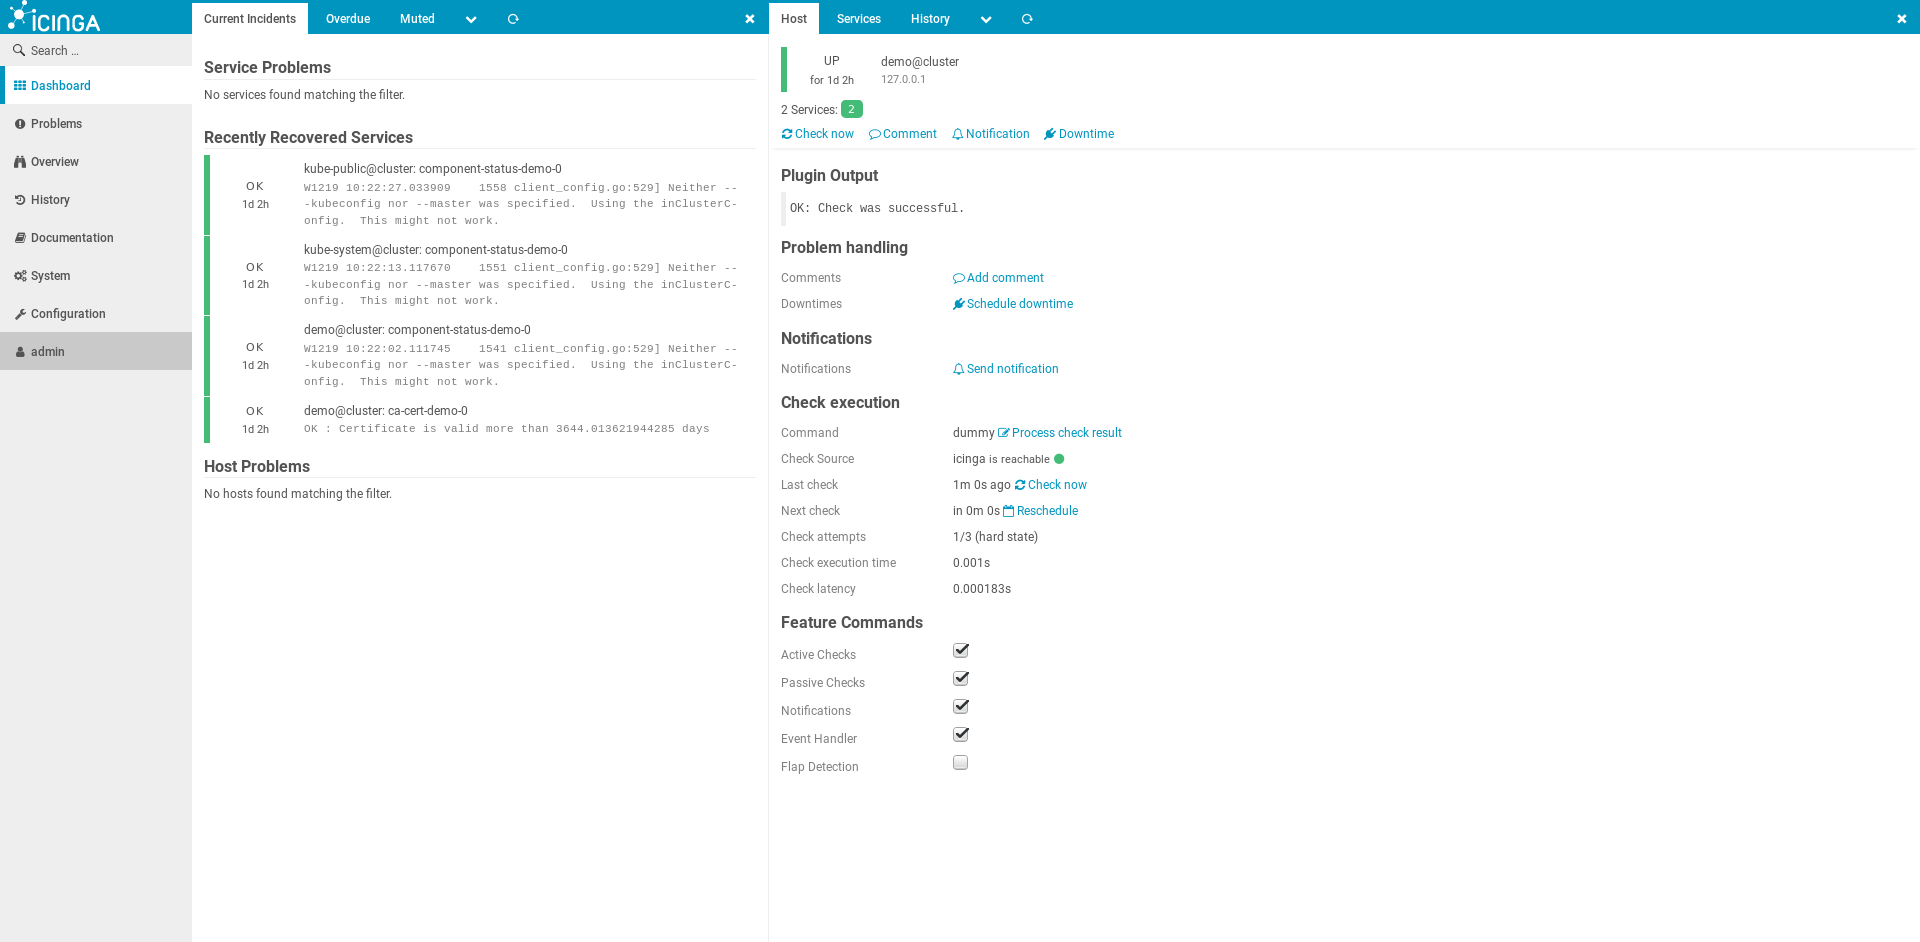
\includegraphics[width=1\linewidth]{Bilder/Searchlight_Icinga}\\
Icinga/Searchlight comes in a  discreet blue/withe coloring. On the dashboard which represents the homepage of the application an overview of the implemented alerts is shown. The alerts are colored with green/yellow/red for OK/warning/error, so it is easy to see appearing problems.\\
 The rest of the options like history and configurations is located at the sidebar. Information about the monitored host and services is located in an extra row, presented on the right.
\subsection{Performance}
In our VM deployment the applications has allocated 160MB of RAM under load. The application it self is running very smooth even on low power systems. As we deployed some alerts, we noticed, that it took about 30 seconds to validate the alert and get a first status from the system. After that pending status everything is running smoothly and even checks on a 30 second rhythm were no problem for the system.
\subsection{Interoperability}
On the Github page \cite{searchlight} of the program the developer claims to be able to send notification over email, SMS and chat.
In the guide there is no explicit explanation what is meant by the term chat but the tool is able to send notifications to Slack \cite{slack} and Hipchat \cite{hipchat}. Notification over email can be send over SMTP without any third party software. To send SMS a service like Twilio \cite{twilio} is needed.
On the page there is no advise that the tool is capable to interact over an interface with other notification than the given. Furthermore the developer gives no interfaces in at all for interaction with other applications.
\subsection{Conclusion}
Searchlight is a light weighted  port of the famous monitoring tool Icinga. It runs well and has all basic needed features. As we had a deeper Look  into the software  it revealed its weakness. There are no advanced possibilities to connect Searchlight with over monitoring tools. Also there is no graphical user interface for creating alerts, which makes it very difficult to set it up. As the tool is manly developed and updated by only two people the support for new versions of Icinga and Kubernetes is limited. The fact that the company Appcode Inc. has no direct correlation with Icinga is another counter-argument to the tool. In a nutshell the tool is good for small Kubernetes clusters that want to monitor only a few basic metrics and have low resources. 

\section{Prometheus}
\label{Prometheus} % to refernce in the document
The tool Prometheus is a open source project and is hosted by the Cloud Native Computing Foundation.
It is a single tool that comes with the features of a whole monitoring stack (without alerting).\\ Prometheus own collector uses client libraries, supported for different languages including GO, Java, Scala, Python and Ruby and more third-party libraries for various other languages. The collector is able to pull data from the server or cluster and can be accessed via HTTP request.
The project was originally built at Soundcloud \cite{soundcloud} and  is nowadays used by big companies like Jodel \cite{jodel}, Docker and Core OS \cite{prometeus}.
Prometheus also has an alert manager, which is an extra tool to send message including the cluster state via email, HipChat, PagerDuty, Pushover, Slack, OpsGenie and VictorOps. These alerts have to be set up by an configuration file. 
Because the project is community driven, there is no official repository for Prometeus on Kubernetes, but with a little research we managed to find a repository \cite{prometheus_kube} that provided different deployments for cloud environments.

\subsection{Installation}
We managed to install Prometheus in a way that we were able to get metrics from the  Kubernetes Api-server and can expose the metrics over a RESTful interface. Over this interface it is possible to connect Prometheus to a application outside or inside the cluster like Grafana, which is recommended for Prometheus by the developers. We were not able to install the Prometheus own alert manger on the cluster. Also we were not able to get metrics from the cluster-nodes because our Prometheus version is not cable of requesting over HTTPS (Hypertext Transfer Protocol Secure), which has to be used for the nodes. 
\subsection{Appearance}%Only for Visual tools
Prometheus provides a web user interface to present the collected data. It is designed in a very light weighted black and a withe combination with some blue accents and only shows the necessary informations. The interface has no function to save the set of graphs that is selected and no option to authenticate, so that the data can be keeped secret. 
\subsection{Performance}
The tool is very quickly booted and shows no Performance problems on the interface. A look on the stats shows that Prometheus is not very CPU dependent, it oscillates up and down because the collection data peaks as show in \cref{fig:Prometeus_Cpu}. In the use of memory the tool is a little bit more demanding and takes up to 2GB of RAM. These high numbers of RAM is allocated over a time from about 24h. 
\begin{figure}
\centering
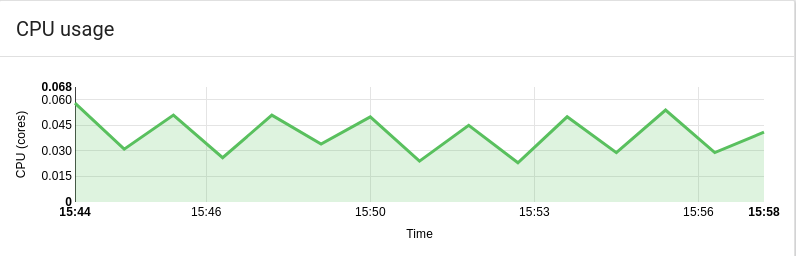
\includegraphics[width=0.5\linewidth]{Bilder/Performance/Prometeus_Cpu}
\caption{CPU usage of Promtheus}
\label{fig:Prometeus_Cpu}
\end{figure}
\subsection{Interoperability}
It is highly recommended that Prometheus is used with a graphing and an alerting tool, due to the fact that it is just a collector and time series database with a query engine. In our deployment Graphana is used for both tasks, because it is the recommended tool from the Prometheus web page \cite{prometheus}. Exploiting Prometheus to any other tool is also possible as Prometheus provides the metrics that are collected in plain text over a RESTful interface.
\subsection{Conclusion}
Prometheus is very good as a collector for large Kubernetes Clusters with hundreds or thousands of nodes. What makes it so good is the with-box monitoring approach, which provides way more metrics than a black-box monitoring. These fact can be used to detect problems in the system earlier and in much more detail so that the downtime can be reduced. On the other side Prometheus is not good for presenting this data and to throw alerts in case of failure.

\section{Zabbix}
\label{Zabbix} % to refernce in the document
% \url{https://dl.acm.org/citation.cfm?id=1883485} Linux Journal
\cite{Hernantes2015}
The tool Zabbix is an open-source tool and is developed by Zabbix LLC (Limited Liability Company) since 2005 \cite{zabbix}. Zabbix provides an all in one solution which includes an collector, a database, a visualization tool and an alert manager.
\subsection{Installation}
There is an repository from monitoringartist \cite{zabbix_kube} that provides diverse yaml files, that map the Zabbix client and server on a cluster structure. The single modules are scalable by the user afterwards in the Cluster. By default 3 copies of the database engine and web user interface are deployed. In the repository are two types of Zabbix deployment. The first we tested uses a load balancer the second one uses the cloud network balancing engine from Google.
\subsection{Appearance}%Only for Visual tools
Zabbix come with a withe and blue web interface with some red accents. It implements a tab system with sub tabs to navigate through the interface. The naming of the tabs is not as self explaining as it could be.  
\subsection{Performance}
The general performance of Zabbix is very good. The three parts take up to 1GB of RAM of the System and about 0.5 \% of the processor load. The minimum requirements of Zabbix are specified with Pentium 2 of 350Mhz and 256MB of Ram \cite{Marik2014}.
\subsection{Interoperability}
Zabbix provides a different API to connect to other entities. The web interface  provides a PHP script that accepts queries and can be configure to use authentications . Grafana has a extra plug-in which is connectible to this script and show a optimized dashboard with all relevant informations. The tool is also capable of sending alerts over email, SMS, and jabber. Zabbix gives also the ability to create custom scripts that execute in case of a alert. For example a cli script can be triggered over ssh. 
\subsection{Conclusion}
Zabbix is one of the best optimized and extended open-source solutions available. The installation was by far the simplest and overarching of all the tested tools. The configuration is complex and the naming is not at every position as expected. By default Zabbix scales over all of the available nodes but can be scaled up manual. The best way to use Zabbix is to pare it with a Grafana instance which provides the information from Zabbix tighter and with a better overview.

\section{ELK Stack }
\label{elk} % to refernce in the document
The ELK stack is developed by elastic \cite{elasticsearch}. 
The stack is a logging tool which is developed java and divided up into three parts. First  logstash and beats with there sub tools like Metric beat or Heartbeat for collecting. Second Elasticsearch which queries the data and makes them persistent and last Kibana the visualization tool of the stack.
\subsection{Logstash/Beats}
Logstash is by elastic described as an 
"server-side data processing pipeline"\cite{elasticsearch}. These piplines a able to process nearly every data (github webhooks, http push/poll, irc, imap ,....).
While collecting the data Logstash already transforms it into data structures for better retrieval.
Beats is a "single-purpose data shipper"\cite{elasticsearch} and more what we understand under the term Collector
\subsection{Elasticsearch}
\label{Elasticsearch}
Due to the elastic company "Elasticsearch is a distributed, RESTful search and analytics engine capable of solving a growing number of use cases"\cite{elasticsearch}.\\ It makes the data persistent in JSON (JavaScript Object Notation) with it is own Query Domain Specific Language. Theses files are named shards and can be spread over multiple Servers.
\subsection{Kibana}
Kibana is a Browser based Open-Source visualization Plugin. It is under the Apache License and is written in JavaScript. It features a web interface with a user login. This gives the owner the power to control who is using which features. User logins can be either added manually or via LDAP.
Kibana offers a lot of different graphs including classic line graphs, data tables, area graphs, pie charts, bar graphs.
\subsection{Installation}
ELK Stack is deployable at the Kubernetes cluster. There is a solution on github provided by Kubernetes. After the installation there 
\subsection{Appearance}%Only for Visual tools
Kibana is the only tool in the complete Stack with a user interface. It is accessible over the homepage of the application. The site is starting with a discover page, where all logs are listed in a time chronological order. The discover page also allows to filter these logs by key words. On the left side is the sidebar with management, devtools, visualize, time line, discoverer and dashboard. The dashboard tab, is for creating an own dashboard with the own preferences.
\subsection{Performance}
The tool stack ELK is booting very fast. As seen in the \cref{fig:ELK_CPU}, the CPU usage is very high at the start, but when all is up, it is running on low CPU usage. At the start the RAM consumption is low but when it starts collecting log data's the amount of used RAM is growing very fast (\cref{fig:ELK_MEM}). The growth was so fast, that our Kubernetes cluster broke after a view days because the server was out of memory.
\begin{figure}
	\centering
	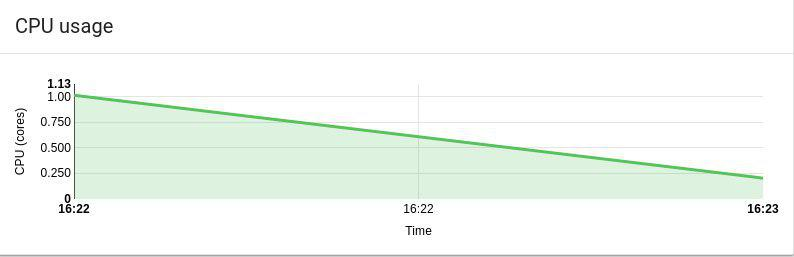
\includegraphics[width=0.5\linewidth]{Bilder/Performance/ELK_CPU}
	\caption{}
	\label{fig:ELK_CPU}
\end{figure}
\begin{figure}
	\centering
	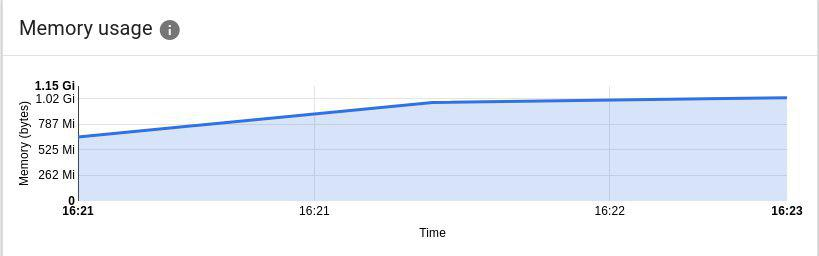
\includegraphics[width=0.5\linewidth]{Bilder/Performance/ELK_MEM}
	\caption{}
	\label{fig:ELK_MEM}
\end{figure}
\subsection{Interoperability}
Elasticsearch also offers a tool to include alerts. The tool can send any alerts which you can query with Elasticsearch. On the official website, elastics mentioned they can send the notifications on E-Mail, PagerDuty, Slack and HipChat and it also offers an interface with an webhook-output to integrate any third-party-software for messaging. With this interface it might be easy to include sending alerts with SMS like earlier mentioned the program Twilio(\ref{searchlight}).
\subsection{Conclusion}


\section{Grafana}
\label{grafana} % to refernce in the document
Grafana is a tool to visualize the data collected about a system. It features different graphs, including graphs with changes over time, single stats for live feeds, tables to show multiple data from different sources and heat maps to show the distribution of values over a timespan.
Grafana also comes with an inbuilt alerting system which allows the user to be notified under specific conditions via E-Mail, Slack, PagerDuty, Kafka. The alerting also has a webhook, allowing the user to send his alerts to a custom endpoint via HTTP.
The graphs and alerts are setup in the web interface of Grafana which comes with it is own user management. It differentiates between users and administrators and super-administrators. Administrators can be assigned to an organization, allowing different systems to be monitored by one Grafana instance, while still giving the owners of the single system the option to manage their own alerts and graphs.
Grafana also features a LDAP Authentication to automatically import users and permissions from a user directory.
\subsection{Installation}
The installation of Grafana is very simple, because it only runs on a single Docker container. Because Grafana is no collector over tools provide an extra version of Grafana in there repository that is optimized for there data sources.
\subsection{Appearance}%Only for Visual tools
Grafana mainly uses the colors red and orange and comes with a dashboard. Due to the data source that is selected this changes to a set of graphs which show the information of the data source. Per drag and drop the graphs and text boxed can be freely moved around. 
\subsection{Performance}
The performance of Grafana is very good. The tools consumes nearly no CPU and only a few megabytes of RAM as shown in \cref{fig:Grafan_RAM}. The Diagram also shows that the amount of the used resources is constant over time
\begin{figure}
\centering
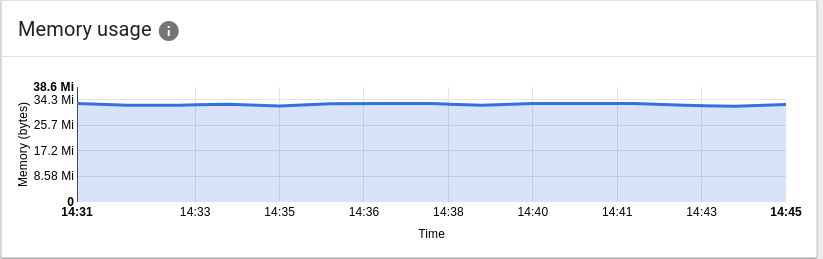
\includegraphics[width=0.5\textwidth]{Bilder/Performance/Grafan_RAM}
\caption{Graphane Ressource use}
\label{fig:Grafan_RAM}
\end{figure}
\subsection{Interoperability}
Grafana can interact with nearly every interface to sent alerts because of it is Web hooks which can send and request to an restful endpoint over a JSON document. Whats special about the alerting engine of Grafana is that pictures can be send within the alerts. The pictures is taken of the Grafana to present the alert in a visual way and can be send with the notification or can be uploaded to services like Amazon S3.

\subsection{Conclusion}
Grafana is by far the best and biggest visualization tool on the open-source market. Due to the capability to write custom plug ins nearly every tool stack has an integration which is easy to install and uses the features of Grafana in the intention of the developer.

\section{TICK}
\label{tick}
TICK is a Monitoring Stack provided by the InfluxData company and is under MIT License which is an Permissive software license.
\subsection{Telegraf}
Telegraf is the data collector of the TICK stack by Influxdata and is written entirely in GO. It is a lightweight data collector as it needs specific plugins for metrics to be collected. These can be chosen by the user as needed for the system. It has official input plug ins for many servers including Apache, Cassandra, Kubernetes, MySQL.
The outputs are also handled by plug ins. This allows the user to send the metrics to almost any endpoint as there is a broad variety of plug ins. As with the input plug ins, there is also a broad variety of output plugins including for Influxdatas own InfluxDB, Elasticsearch(\ref{Elasticsearch}) from the ELK Stack, Prometheus(\ref{Prometheus}). It also supports more primitive outputs like writing to file or TCP/UDP Socket.
\subsection{InfluxDB}
InfluxDB is the time-series database from the TICK stack by Influxdata. It is written in GO and available as a single binary with no external dependencies. This makes the installation, as either a standalone database or as a Kubernetes pod, simple.
By default it supports their own collector, Telegraf, but other collectors are supported via plug ins. The data can be written with their  HTTP/S API using it is own SQL-like query language, InfluxQL, which also gives the option of creating your own interfaces.
To minimize storage consumption data will be down sampled over time. The recent high precision data is stored in the database only for a limited time and then summarized with other data to keep hard-drive usage reasonable. 
\subsection{Chronograf}
Chronograf is the Visualization Tool of the TICK Stack by Influxdata. It comes with a web interface to display all the data collected by Telegraf. Data can be visualized in different graph-types including single and stack line graphs, Step-Plot, Single stat and bar graphs. It comes with a lot of pre-configured dashboards for all the applications which are also officially supported by Telegraf, though it is also possible to create your own dashboards or modify the existing ones. 
Chronograf also features a UI for Influxdatas own alerting tool Kapacitor, which allows the management of both tools in one interface.
\subsection{Kapacitor}
Kapacitor is the Alerting Tool of the TICK Stack by Influxdata. Various alerts can already be defined when using Chronograf with Kapacitor including static thresholds, percentage values and Deadman switches. It also supports more complex alert conditions via TICKscripts which have to be defined in Kapacitor directly.
The alerts it self can then be sent to various endpoints like HipChat, Pagerduty, Pushover, Slack, Telegram and many more. It also supports more simplistic endpoints like file outputs, TCP sockets or HTTP Post.
Kapacitor does not feature a web interface as it is meant to be used with Chronograf which already has a UI component for Kapacitor. It can be used without this interface via console inputs.
\subsection{Installation}
The installation of the TICK stack in special Telegraf and Influxdb is very simple. A possible portation of the tool is delivered by the developer of Kubernetes in there Github repository Heapster \cite{heapster}. Heapster is used by the stack to collect the monitoring information of the pods in one place.
\subsection{Appearance}
Only Chronograf provides a web interface for the user. The interface is in blue withe combination and contains a lot of black. The menu is located on an left sidebar but there are only symbols. On hover the text appears and shows further informations for navigation. It offers a graphical way to inject alerts into Kibana.

\subsection{Performance}
In our cluster the TICK stack performed very well which matches the InfluxData guidelines that recommend a dual core CPU and 2 to 4 gb of RAM \cref{fig:TICK_recommendet} as minimum and for system with under five queries per second. Due to the Developer TICK can handle up to over 100 queries but then need 4 to 8 times more resources \cite{influx_require}.
\begin{figure}
\centering
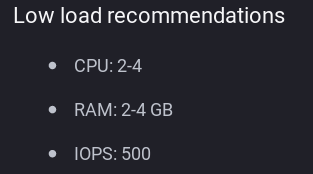
\includegraphics[width=0.35\textwidth]{Bilder/Performance/TICK_recommendet}
\caption{Graphane Ressource use}
\label{fig:TICK_recommendet}
\end{figure}

\subsection{Interoperability}
TICK and in special influxdb can be accessed by many tools. Because TICK stack is very common many tools offer plug-in integrations. In special we tested Grafana because it is recommended by the developer and integrates out of the box. Influx exposes to it not only the physical specs of all nodes, but also the stats collected by Kubernetes to every deployed pod. 
\subsection{Conclusion}
The TICK stack is one of the best optimized monitoring solutions for Kubernetes. What makes it special is that information about every running pod instance is collected and can be accessed.



\section{Failed Tools}%Ebenfalls nur ein arbeitstitel
In the process of developing and evaluating the APM we discovered a bunch of tools that we were not able to install even that they claimed to be optimized to work on Kubernetes .
In this paragraph all the tools we wanted to include in our report but does not work, are mentioned with a quick description of the failure.
\subsection{Graphite}
Graphite is mainly for storing and graphing data and metrics, but brings also tools that are able to collect these metrics from the system. By the developer it self there is no Kubernetes installation provided but there are diverse approaches by third party members to make it runnable on a Cluster. We have tested the Repository from nanit \cite{graphite} to get Graphite running with StatsD \cite{statsd} as a metric collection tool. The Repository does not provide a yaml file by it self to install all the tools. The instruction leads the user to export some variables needed for the installation. After that a deploy command is provided that pulls the docker repository and than installs it with kubectl on the Cluster. As we tried to execute this command an error was thrown, The node replicas were empty, so no further commands are executable. As we were not able to install the tool on multiple Kubernetes Clusters, we installed the tool as on the website advertised on a Ubuntu system directly. With this installation of Graphit a time-series data, an monitoring and alerting tool is included. On the test system the monitoring system gave values that differs from the Linux intern monitoring in values like CPU usage or RAM. As a solution to all this difficulties we decided to not perform further test on the tool.

\subsection{Icinga}
\label{Icinga}
Icinga is as ELK-Stack not a monitoring tool. Its made for logging defined requests. The administrator can decide which system to monitor and in what interval the data is pulled.
Icinga it self only provides 3 system states instead of exact values. The states are OK/warning and error. The user decides at which point they are triggered.\\
As we tried to install Icinga we found out that there was no direct support from Incinga for Kubernetes. As our Study only describes the actual state without trying to add something we decided not to try an compile Icinga into Kuberntes on our own. Later we found out there is a third party Software called searchlight \ref{searchlight} which is provided by Appscode on Github.
 